% computing position and velocity of satellite
\section{卫星位置}

\subsection{坐标系}
\begin{frame}{常用坐标系}
    \begin{itemize}[<+-| alert@+>]
        \item 地心地固直角坐标系$\left( \mathrm{ECEF} \right)$
        \begin{itemize}
            \item[] 地心为坐标原点, $OZ$指向北极, $OX$指向参考子午面与地球赤道的交点
        \end{itemize}
        \item 经纬高坐标系$\left( \mathrm{ LLA } \right)$
        \begin{itemize}
            \item[] 地心为坐标原点, 大地高度$h$是过该点到基准椭球面的法线距离
        \end{itemize}
        \item 站心坐标系$\left( \mathrm{ ENU } \right)$
        \begin{itemize}
            \item[] 观测点为坐标原点, 三坐标轴分别指向东, 北, 天方向
        \end{itemize}
    \end{itemize}
\end{frame}

\begin{frame}{坐标变化}
    \begin{itemize}
        \item $\mathrm{LLA} \rightarrow \mathrm{ECEF}$
        \begin{align*}
            x &= \left( N + h \right) \cos \varphi \cos \lambda \\
            y &= \left( N + h \right) \cos \varphi \sin \lambda \\
            z &= \left[ N \left( 1 - \mathrm e ^ 2 \right) + h \right] \sin \varphi
        \end{align*}
        其中,
        \begin{align*}
            \mathrm e &= \sqrt{ 1 - \frac{ b ^ 2 }{ a ^ 2 } } \\
            N &= \frac{ a }{ \sqrt{ 1 - \mathrm e ^ 2 \sin ^ 2 \varphi } }
        \end{align*}
    \end{itemize}
\end{frame}

\begin{frame}{坐标变换}
    \begin{itemize}
        \item $\mathrm{ECEF} \rightarrow \mathrm{LLA}$
        \begin{align*}
            \lambda &= \arctan \frac{ y }{ x } \\
            h &= \frac{ \sqrt{ x ^ 2 + y ^ 2 } }{ \cos \varphi } - N \\
            \varphi &= \arctan \left[ \frac{ z }{ \sqrt{ x ^ 2 + y ^ 2 } }
            \left( 1 - \mathrm e ^ 2 \frac{ N }{ N + h } \right) ^ { -1 }\right]
        \end{align*}
        其中, $h$与$\varphi$组成耦合非线性方程组, 采用迭代方法求解.
    \end{itemize}
\end{frame}

\subsection{星历文件}
\begin{frame}{星历文件主要参数}
\begin{table}[h!]
    \centering
    \footnotesize
    \caption{星历文件参数}
    \begin{tabular}{ccc}
        \hline
        $t _ { 0e }$ && 星历参考时刻 \\
        $\sqrt{ a }$ && 轨道半长轴的平方根 \\
        $e$ && 轨道离心率 \\
        $i _ 0$ && $t _ { 0e }$时刻轨道倾角 \\
        $\Omega _ 0$ && 升交点经度 \\
        $\omega$ && $t _ { 0e }$时刻近地点幅角 \\
        $M _ 0$ && $t _ { 0e }$时刻平近点角 \\
        $\mathrm d i / \mathrm d t$ && 倾角变化率 \\
        $\mathrm d \Omega / \mathrm d t$ && 升交点经度变化率 \\
        $\Delta n$ && 平均角速度的校正值 \\
        $C _ { uc }$ && 维度幅角余弦修正值 \\
        $C _ { us }$ && 维度幅角正弦修正值 \\
        $C _ { rc }$ && 轨道半径余弦修正值 \\
        $C _ { rs }$ && 轨道半径正弦修正值 \\
        $C _ { ic }$ && 倾角余弦修正值 \\
        $C _ { is }$ && 倾角正弦修正值 \\
        \hline
    \end{tabular}
    \label{tab:ephemeris_para}
\end{table}
\end{frame}

\begin{frame}{计算卫星位置}
    \begin{figure}
        \centering
        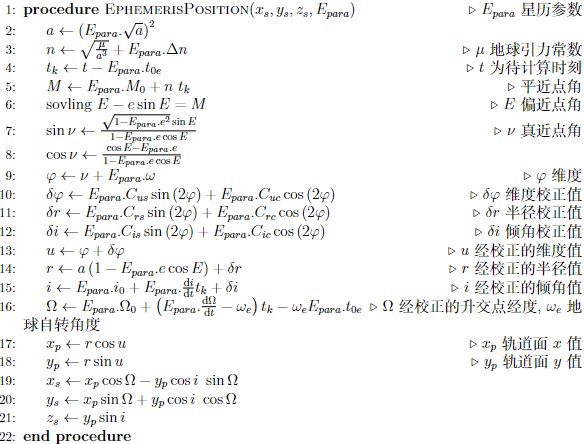
\includegraphics[width = .7\textwidth]{pic/algo_ephemeris.jpg}
        \label{fig:alg_ephemeris}
    \end{figure}
\end{frame}

% computing distance
\section{距离}

\subsection{伪距模型}
\begin{frame}{伪距}
    \begin{itemize}
        \item 接收机钟差$\delta _ t ^ A$, 卫星钟差$\delta _ t ^ { S _ i }$
        \item 卫星信号发射时间$t _ s ^ { S _ i }$, 接收机信号接收时间$t _ u ^ A$
        \begin{align*}
            \rho _ u ^ { S _ i } &= c \left( t _ u ^ A - t _ s ^ { S _ i } \right)
        \end{align*}
        \item 电离层延时$I ^ { S _ i }$, 对流程延时$T ^ { S _ i }$
        \begin{align*}
            \rho _ { I + T } ^ { S _ i } &= c \left( I ^ { S _ i } + T ^ { S _ i } \right)
        \end{align*}
        \item 噪声延时$\varepsilon _ P ^ { S _ i }$
        \begin{align*}
            \rho _ {\varepsilon _ P} ^ { S _ i } &= c \varepsilon _ P ^ { S _ i }
        \end{align*}
    \end{itemize}
\end{frame}

\begin{frame}{接收机与卫星几何距离$\rho _ A ^ { S _ i }$}
    \begin{itemize}
        \item $A \left( x _ A, y _ A, z _ A \right)$与
        $S _ i \left( x _ S ^ i, y _ S ^ i, z _ S ^ i \right)$几何距离
        \begin{align*}
            \rho _ A ^ { S _ i } &= \sqrt{ \left( x _ A - x _ S ^ i \right) ^ 2 
            + \left( y _ A - y _ S ^ i \right) ^ 2 
            + \left( z _ A - z _ S ^ i \right) ^ 2 } \\
            &= c \left[ \left( t _ u ^ A - \delta _ t ^ A \right)
            - \left( t _ s ^ { S _ i } - \delta _ t ^ { S _ i } \right)
            - \left( I ^ { S _ i } + T ^ { S _ i } \right)
            - \varepsilon _ P ^ { S _ i } \right] \\
            &= \rho _ u ^ { S _ i } + c \delta _ t ^ { S _ i }
            - \rho _ { I + T } ^ { S _ i } - \rho _ {\varepsilon _ P} ^ { S _ i } - c \delta _ t ^ A
        \end{align*} \pause
        \item 位置方程表述如下
        \begin{align*}
            \rho _ A ^ { S _ i } + c \delta _ t ^ A &= \rho _ u ^ { S _ i } + c \delta _ t ^ { S _ i }
            - \rho _ { I + T } ^ { S _ i } - \rho _ {\varepsilon _ P} ^ { S _ i }, \ i = 1, 2, \ldots
        \end{align*}
    \end{itemize}
\end{frame}

\subsection{载波相位模型}
\begin{frame}{载波相位}
    \begin{itemize}
        \item 接收机复制的卫星载波信号相位$\phi _ u ^ A$, 接收机接收到的
        卫星载波信号相位$\phi _ s ^ { S _ i }$, 电磁波在此过程中传播的周期数
        为$N _ A ^ { S _ i }$, 无误差的情况下, 卫星与接收机之间的距离$R _ A ^ { S _ i }$
        \begin{align*}
            R _ A ^ { S _ i } &= \lambda _ L \left( \phi _ u ^ A 
            - \phi _ s ^ { S _ i } + N _ A ^ { S _ i } \right)
        \end{align*}
        \item 误差项
        \begin{itemize}
            \item 电离层延时$I ^ { S _ i }$, 对流层延时$T ^ { S _ i }$
            \item 接收机钟差$\delta _ t ^ A$, 卫星钟差$\delta _ t ^ { S _ i }$
            \item 噪声延时$\varepsilon _ \phi ^ { S _ i }$
        \end{itemize}
    \end{itemize}
\end{frame}

\begin{frame}{载波相位模型}
    \begin{itemize}
        \item 初始相位
        \begin{align*}
            \phi _ { u, 0 } ^ A &= \phi _ u ^ A \left( t _ 0 \right) \\
            \phi _ { s, 0 } ^ { S _ i } &= \phi _ s ^ { S _ i } \left( t _ 0 \right)
        \end{align*}
        \item 相位差
        \begin{align*}
            \phi _ A ^ { S _ i } &= \phi _ u ^ A \left( t _ u ^ A \right)
            - \phi _ s ^ { S _ i } \left( t _ s ^ { S _ i } \right) 
            + \frac{ c }{ \lambda _ L } I ^ { S _ i } - \frac{ c }{ \lambda _ L } T ^ { S _ i }
            + N _ A ^ { S _ i }
            - \varepsilon _ \phi ^ { S _ i } \\
            &= \left[ \frac{ c }{ \lambda _ L } \left( t _ u ^ A 
            - \delta _ t ^ A - t _ 0 \right)  + \phi _ { u, 0 } ^ A \right] 
            - \left[ \frac{ c }{ \lambda _ L } \left( t _ s ^ { S _ i } 
            - \delta _ t ^ { S _ i } - t _ o \right) + \phi _ { s, 0 } ^ { S _ i } \right] \\
            &+ N _ A ^ { S _ i } + \frac{ c }{ \lambda _ L } I ^ { S _ i } 
            - \frac{ c }{ \lambda _ L } T ^ { S _ i }
            - \varepsilon _ \phi ^ { S _ i }
        \end{align*}
    \end{itemize}
\end{frame}

\begin{frame}{接收机与卫星几何距离$\rho _ A ^ { S _ i }$}
    \begin{itemize}
        \item $A \left( x _ A, y _ A, z _ A \right)$与
        $S _ i \left( x _ S ^ i, y _ S ^ i, z _ S ^ i \right)$几何距离
        \begin{align*}
            \rho _ A ^ { S _ i } &= \sqrt{ \left( x _ A - x _ S ^ i \right) ^ 2 
            + \left( y _ A - y _ S ^ i \right) ^ 2 
            + \left( z _ A - z _ S ^ i \right) ^ 2 } \\
            &= \lambda _ L \phi _ A ^ { S _ i } \\
            &= c \left( t _ u ^ A - t _ s ^ { S _ i } \right) 
            - c \left( \delta _ t ^ A - \delta _ t ^ { S _ i } \right) 
            + \lambda _ L N _ A ^ { S _ i }
            - \lambda _ L \varepsilon _ \phi ^ { S _ i } \\
            &+ c \left( I ^ { S _ i } - T ^ { S _ i } \right) \\
            &= \rho _ u ^ { S _ i } - c \left( \delta _ t ^ A - \delta _ t ^ { S _ i } \right) 
            + \rho _ { I - T } ^ { S _ i } - \rho _ { \varepsilon _ \phi } ^ { S _ i }
            + \lambda _ L N _ A ^ { S _ i }
        \end{align*}
    \end{itemize}
\end{frame}

\begin{frame}{Remarks}
    \begin{itemize}
        \item 伪距模型$\rho _ A ^ { S _ i }$
        \begin{align*}
            \rho _ A ^ { S _ i } &= \rho _ u ^ { S _ i } - c \left( \delta _ t ^ A 
            - \delta _ t ^ { S _ i } \right)
            - \rho _ { I + T } ^ { S _ i } - \rho _ {\varepsilon _ P} ^ { S _ i }
        \end{align*}
        \item 载波相位模型$\rho _ A ^ { S _ i }$
        \begin{align*}
            \rho _ A ^ { S _ i } &= \rho _ u ^ { S _ i } - c \left( \delta _ t ^ A 
            - \delta _ t ^ { S _ i } \right) 
            + \rho _ { I - T } ^ { S _ i } - \rho _ { \varepsilon _ \phi } ^ { S _ i }
            + \lambda _ L N _ A ^ { S _ i }
        \end{align*}
        \item 伪距与载波相位相结合, 不同测量时刻取差分, 消去周整模糊度
    \end{itemize}
\end{frame}

% solving control equation
\section{求解位置方程}

\subsection{Newton迭代法}
\begin{frame}{Newton迭代格式}
    \begin{itemize}
        \item 位置方程, 未知量$\left[ x _ A, y _ A, z _ A, \delta _ t ^ A \right] ^ \top$
        \begin{align*}
            \left\| x _ A - x _ S ^ 1, y _ A - y _ S ^ 1, z _ A - z _ S ^ 1 \right\| _ 2 
            + c \delta _ t ^ A &= \tilde \rho _ 1 \\
            &\vdots \\
            \left\| x _ A - x _ S ^ n, y _ A - y _ S ^ n, z _ A - z _ S ^ n \right\| _ 2 
            + c \delta _ t ^ A &= \tilde \rho _ n \\
        \end{align*}
        \item 记$f _ i \left( x _ A, y _ A, z _ A, \delta _ t ^ A \right) = \tilde \rho _ i$
        \begin{align*}
            f _ 1 \left( x _ A, y _ A, z _ A, \delta _ t ^ A \right) &= \tilde \rho _ 1 \\
            &\vdots \\
            f _ n \left( x _ A, y _ A, z _ A, \delta _ t ^ A \right) &= \tilde \rho _ n \\
        \end{align*}
    \end{itemize}
\end{frame}

\begin{frame}{Newton迭代格式}
    \begin{itemize}
        \item[1] 迭代初值$\left[ x _ A ^ { (0) }, y _ A ^ { (0) }, z _ A ^ { (0) },
        \left\{ \delta _ t ^ A \right\} ^ { (0) }  \right] ^ \top$
        \item[2] 迭代格式, 记$u ^ { (k) } = \left[ x _ A ^ { (k) }, y _ A ^ { (k) },
        z _ A ^ { (k) }, \left\{ \delta _ t ^ A \right\} ^ { (k) } \right] ^ \top$
        \begin{align*}
            u ^ { ( k + 1 ) } &= u ^ { ( k ) } - J ^ { -1 } \left( u ^ { ( k ) } \right)
            F \left( u ^ { ( k ) } \right),
            \ k = 0, 1, \ldots
        \end{align*}
        \item[3] 满足收敛条件, 迭代终止
    \end{itemize}
\end{frame}

\begin{frame}{Jacobi矩阵}
    \begin{itemize}
        \item 迭代格式中的$J \left( u \right)$定义如下
        \begin{align*}
            J &=
            \begin{bmatrix}
                    \frac{ \partial f _ 1 }{ \partial u _ 1 } & \ldots & 
                    \frac{ \partial f _ 1 }{ \partial u _ 4 } \\
                    \frac{ \partial f _ 2 }{ \partial u _ 1 } & \ldots & 
                    \frac{ \partial f _ 2 }{ \partial u _ 4 } \\
                    \vdots & & \vdots \\
                    \frac{ \partial f _ n }{ \partial u _ 1 } & \ldots &
                    \frac{ \partial f _ n }{ \partial u _ 4 }
            \end{bmatrix}
        \end{align*}
        \item 迭代格式求解
        \begin{align*}
            J \left( u ^ { ( k ) } \right) \left( u ^ { ( k + 1 ) - u ^ { ( k ) } } \right) 
            &= F \left( u ^ { ( k ) } \right), \ k = 0, 1, \ldots
        \end{align*}
        可求解此式的最小二乘解.
    \end{itemize}
\end{frame}
